\section{Hardware}

The hardware used to run the system is heterogeneous and we will show in details
the machines involved in the project.

First of all, we used a desktop pc as a ground station. It specifics are listed below:
\begin{itemize}
  \item Processor: Intel Core(TM) i5-6500 CPU @ 3.20GHz
  \item Memory: 16 GB
  \item Network: Intel Gigabit CT Network Adapter
  \item Storage: 230 GB
\end{itemize}

On this machine, we run a virtual machine which has the following specifics:
\begin{itemize}
  \item Processor: 1 Core
  \item Memory: 4 GB
  \item Storage 25 GB
  \item Network: Virtual adapter
\end{itemize}

The flying vehicles involved in the mission are of two kinds, but both adopt the
same general configuration, even with different hardware. Indeed, they are equipped
with a flight control unit connected with a companion microcomputer by the serial port.
The microcomputer communicates with the ground station using the Wifi.

\subsection{Pixfalcon}
The flight control unit adopted is the Pixfalcon (figure \ref{fig:hardware_pixfalcon})
which belongs to the family of the Pixhawk \cite{pixhawk}.

\begin{figure}[h]
\centering
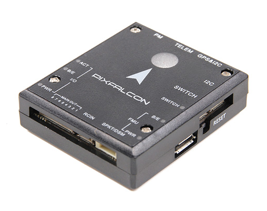
\includegraphics[width=0.35\textwidth]{chapters/chapter-03/figures/hardware_pixfalcon.png}
\caption{Pixfalcon board}
\label{fig:hardware_pixfalcon}
\end{figure}

Its specifications are the following:
\begin{itemize}
  \item Main System-on-Chip: STM32F427
        \begin{itemize}
          \item CPU: 180 MHz ARM Cortex M4 with single-precision FPU
          \item RAM: 256 KB SRAM (L1)
        \end{itemize}

  \item Failsafe System-on-Chip: STM32F100
        \begin{itemize}
          \item CPU: 24 MHz ARM Cortex M3
          \item RAM: 8 KB SRAM
        \end{itemize}

  \item Wifi: ESP8266 external
  \item GPS: U-Blox 7/8 (Hobbyking) / U-Blox 6 (3D Robotics)
  \item Connectivity:
    \begin{itemize}
      \item 1x I2C
      \item 1x CAN (2x optional)
      \item 1x ADC
      \item 4x UART (2x with flow control)
      \item 1x Console
      \item 8x PWM with manual override
      \item 6x PWM / GPIO / PWM input
      \item S.BUS / PPM / Spektrum input
      \item S.BUS output
    \end{itemize}
\end{itemize}

\subsection{Intel Edison}
The companion computers are of two types.
The first kind is the Intel Edison \cite{edison} (figure \ref{fig:hardware_edison})
which is a general purpose computer.

\begin{figure}[h]
\centering
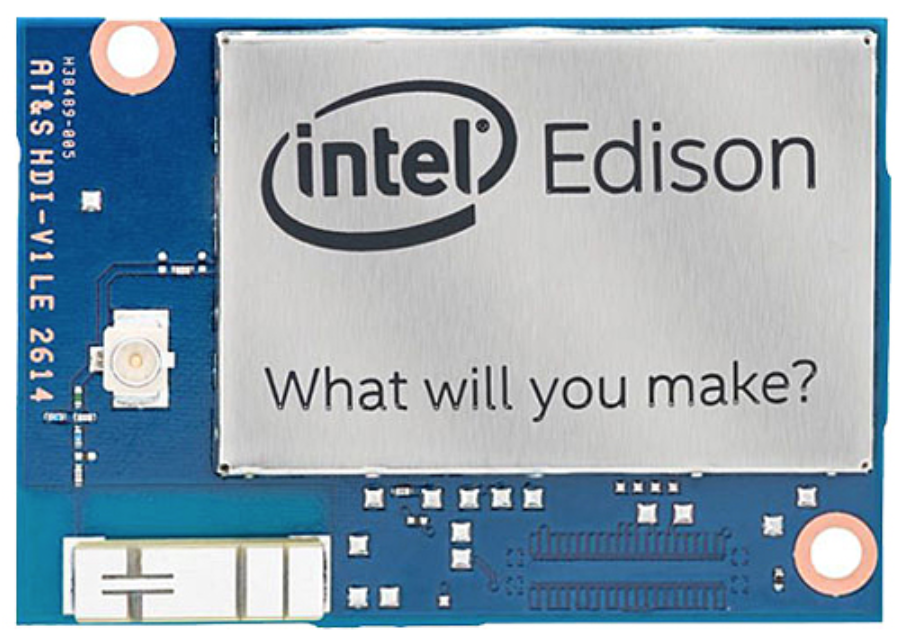
\includegraphics[width=0.35\textwidth]{chapters/chapter-03/figures/hardware_edison.png}
\caption{Edison board}
\label{fig:hardware_edison}
\end{figure}

The specifications are the following:

\begin{itemize}
  \item Atom 2-Core (Silvermont) x86 @ 500 MHz
  \item Memory: LPDDR3 1 GB
  \item Storage: 4 GB EMMC
\end{itemize}

\subsection{RaspberryPi Zero}
The second kind of companion is the RaspberryPi Zero \cite{raspberry}
(figure \ref{fig:hardware_raspberry}).

\begin{figure}[h]
\centering
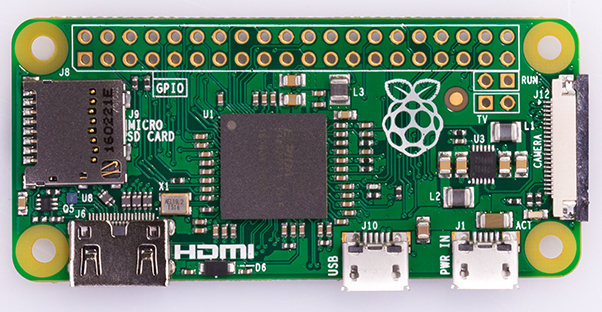
\includegraphics[width=0.35\textwidth]{chapters/chapter-03/figures/hardware_raspberry.jpg}
\caption{RaspberryPi Zero board}
\label{fig:hardware_raspberry}
\end{figure}

Its specifications are the following:

\begin{itemize}
  \item Processor:
        \begin{itemize}
          \item Broadcom BCM2835
          \item contains an ARM1176JZFS (ARM11 using an ARMv6-architecture core)
        \end{itemize}

  \item Memory: 512MB LPDDR2 SDRAM
  \item USB On-The-Go port
  \item Mini HDMI
  \item 40pin GPIO header
  \item CSI camera connector
\end{itemize}

\subsection{Motive Optitrack}
The motion capture system is Motive Optitrack \cite{optitrack}.
We use eight Optitrack Prime 13 cameras \cite{prime13},
arranged on a square as show in the figure \ref{fig:camera_square}. 
The defined volume is a cube of 5 meters per side,
and the drones can fly without obstacles inside it.

\begin{figure}[h]
\centering
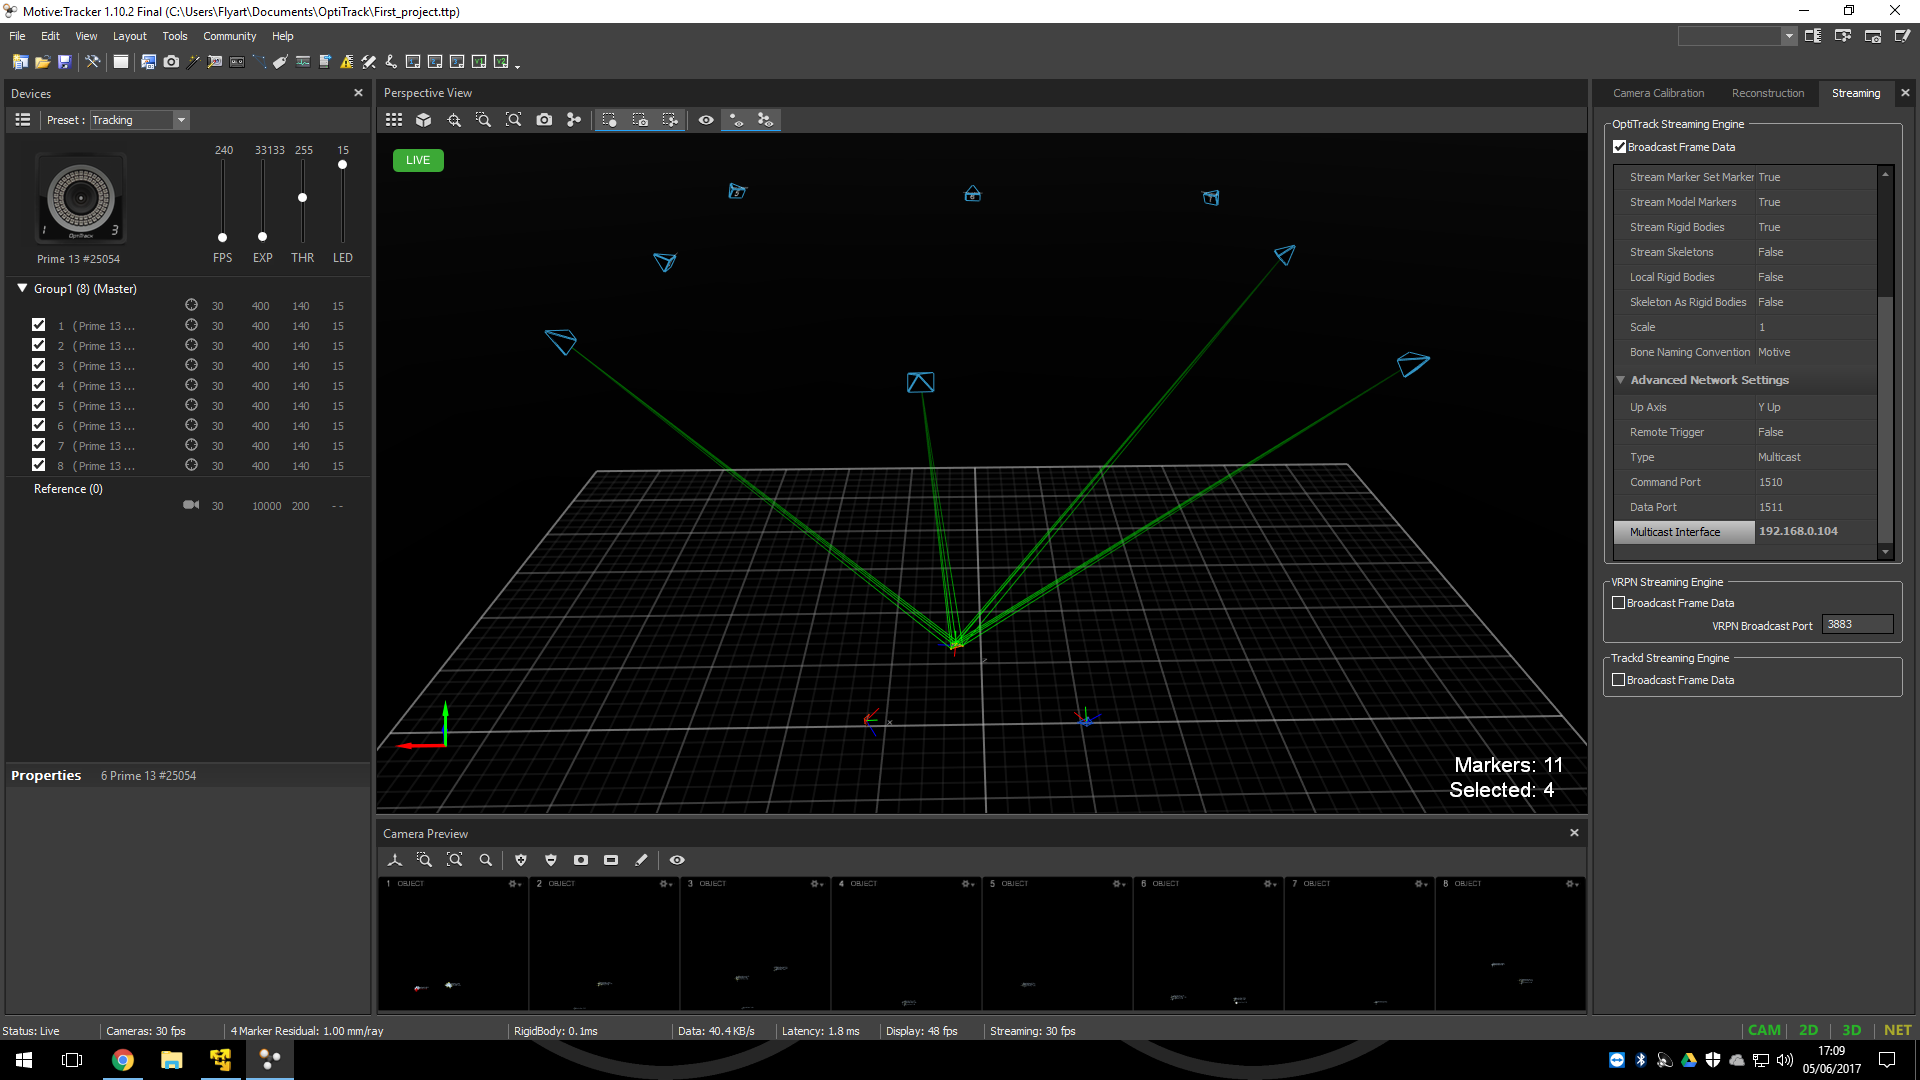
\includegraphics[width=1.0\textwidth]{chapters/chapter-03/figures/cameras_square.png}
\caption{Motive Optitrack screenshot}
\label{fig:camera_square}
\end{figure}

The cameras are connected to a Netgear Prosafe 28PT GE POE \cite{netgear} switch using
Gigabit Ethernet cables.

In order to be visible by the Optitrack system, every drone must be equipped with
markers (figure \ref{fig:marker}) with different configurations,
which make possible the diversification of all the drones.

\begin{figure}[h]
\centering
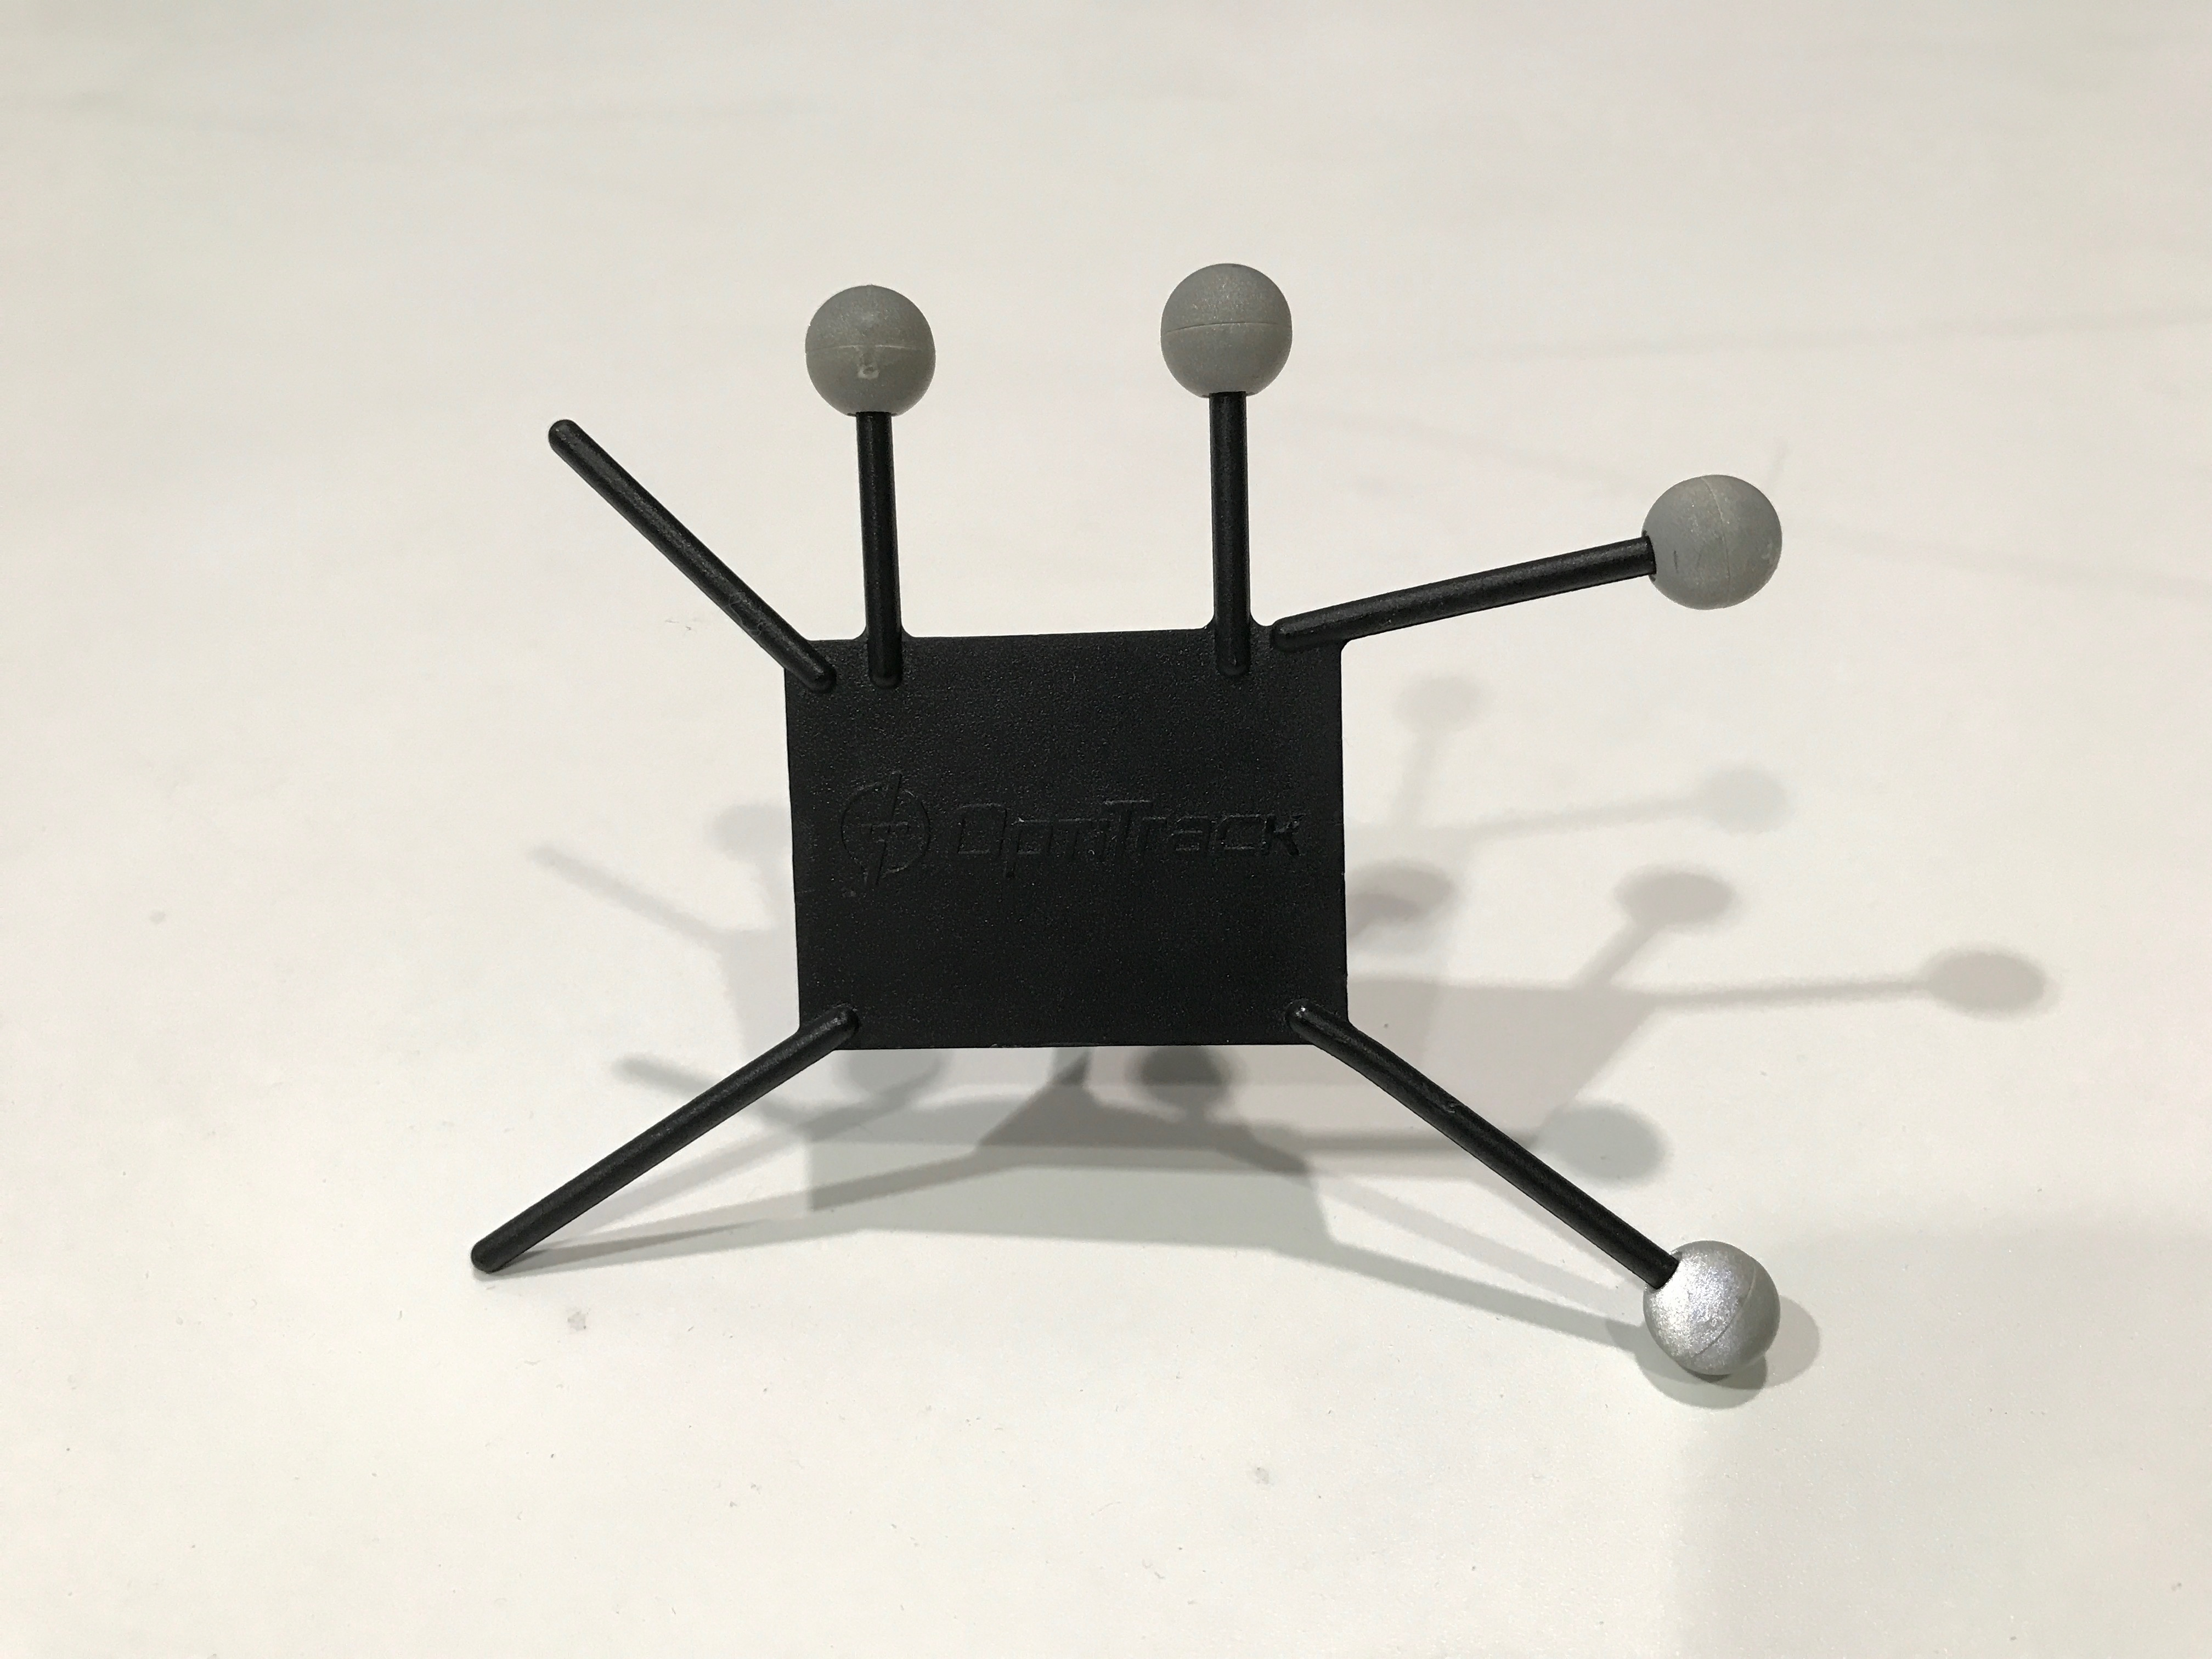
\includegraphics[width=0.7\textwidth]{chapters/chapter-03/figures/marker.jpg}
\caption{Optitrack marker}
\label{fig:marker}
\end{figure}

The two models of drone which we will use are presented in the figures \ref{fig:ant1}
and \ref{fig:hexa}. The first one is the Ant model, which is equipped with the Raspberry
Pi Zero and the Pixfalcon. It is a tiny drones which weights about 200g.
The second one is the Hexa model. It is provided with the Intel Edison board and
the Pixfalcon. It is larger and its diameters is about 40cm long.
As we can see from the figures, the Ant model has four propellers, while the Hexa
is provided with six ones.

\begin{figure}[!htb]
\minipage{0.5\textwidth}
  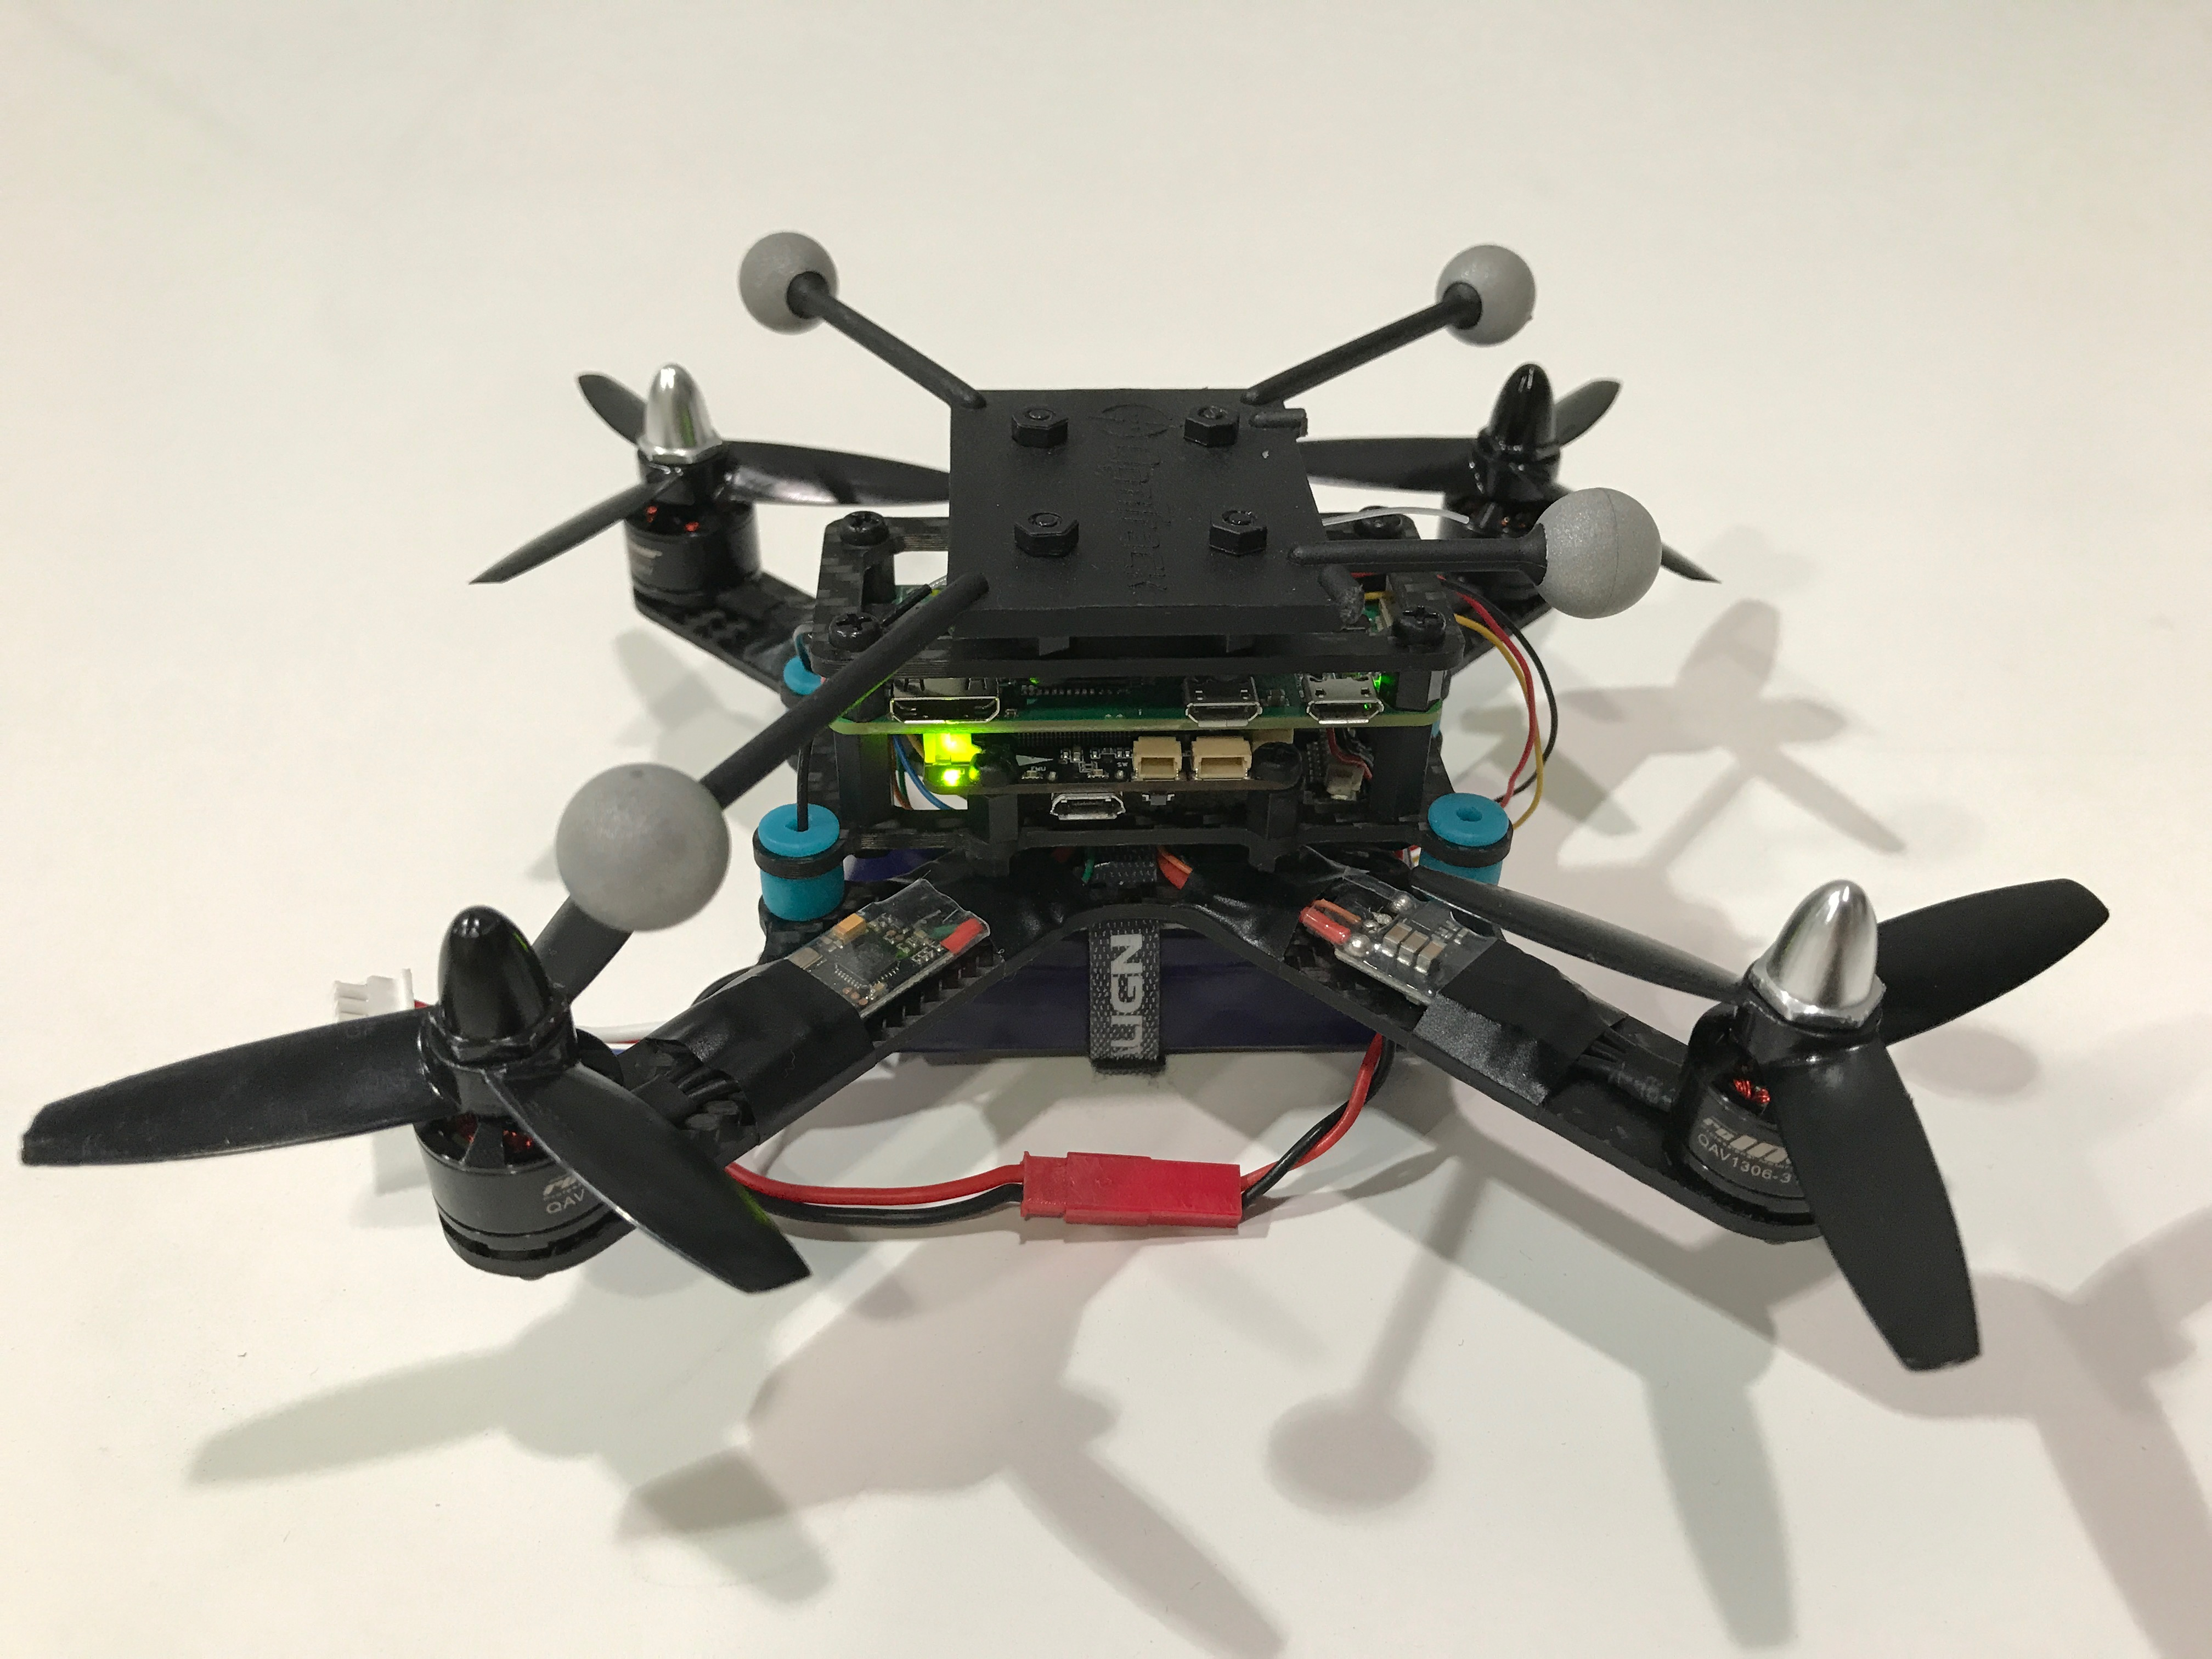
\includegraphics[width=\linewidth]{chapters/chapter-03/figures/ant1_1.jpg}
\endminipage\hfill
\minipage{0.5\textwidth}
  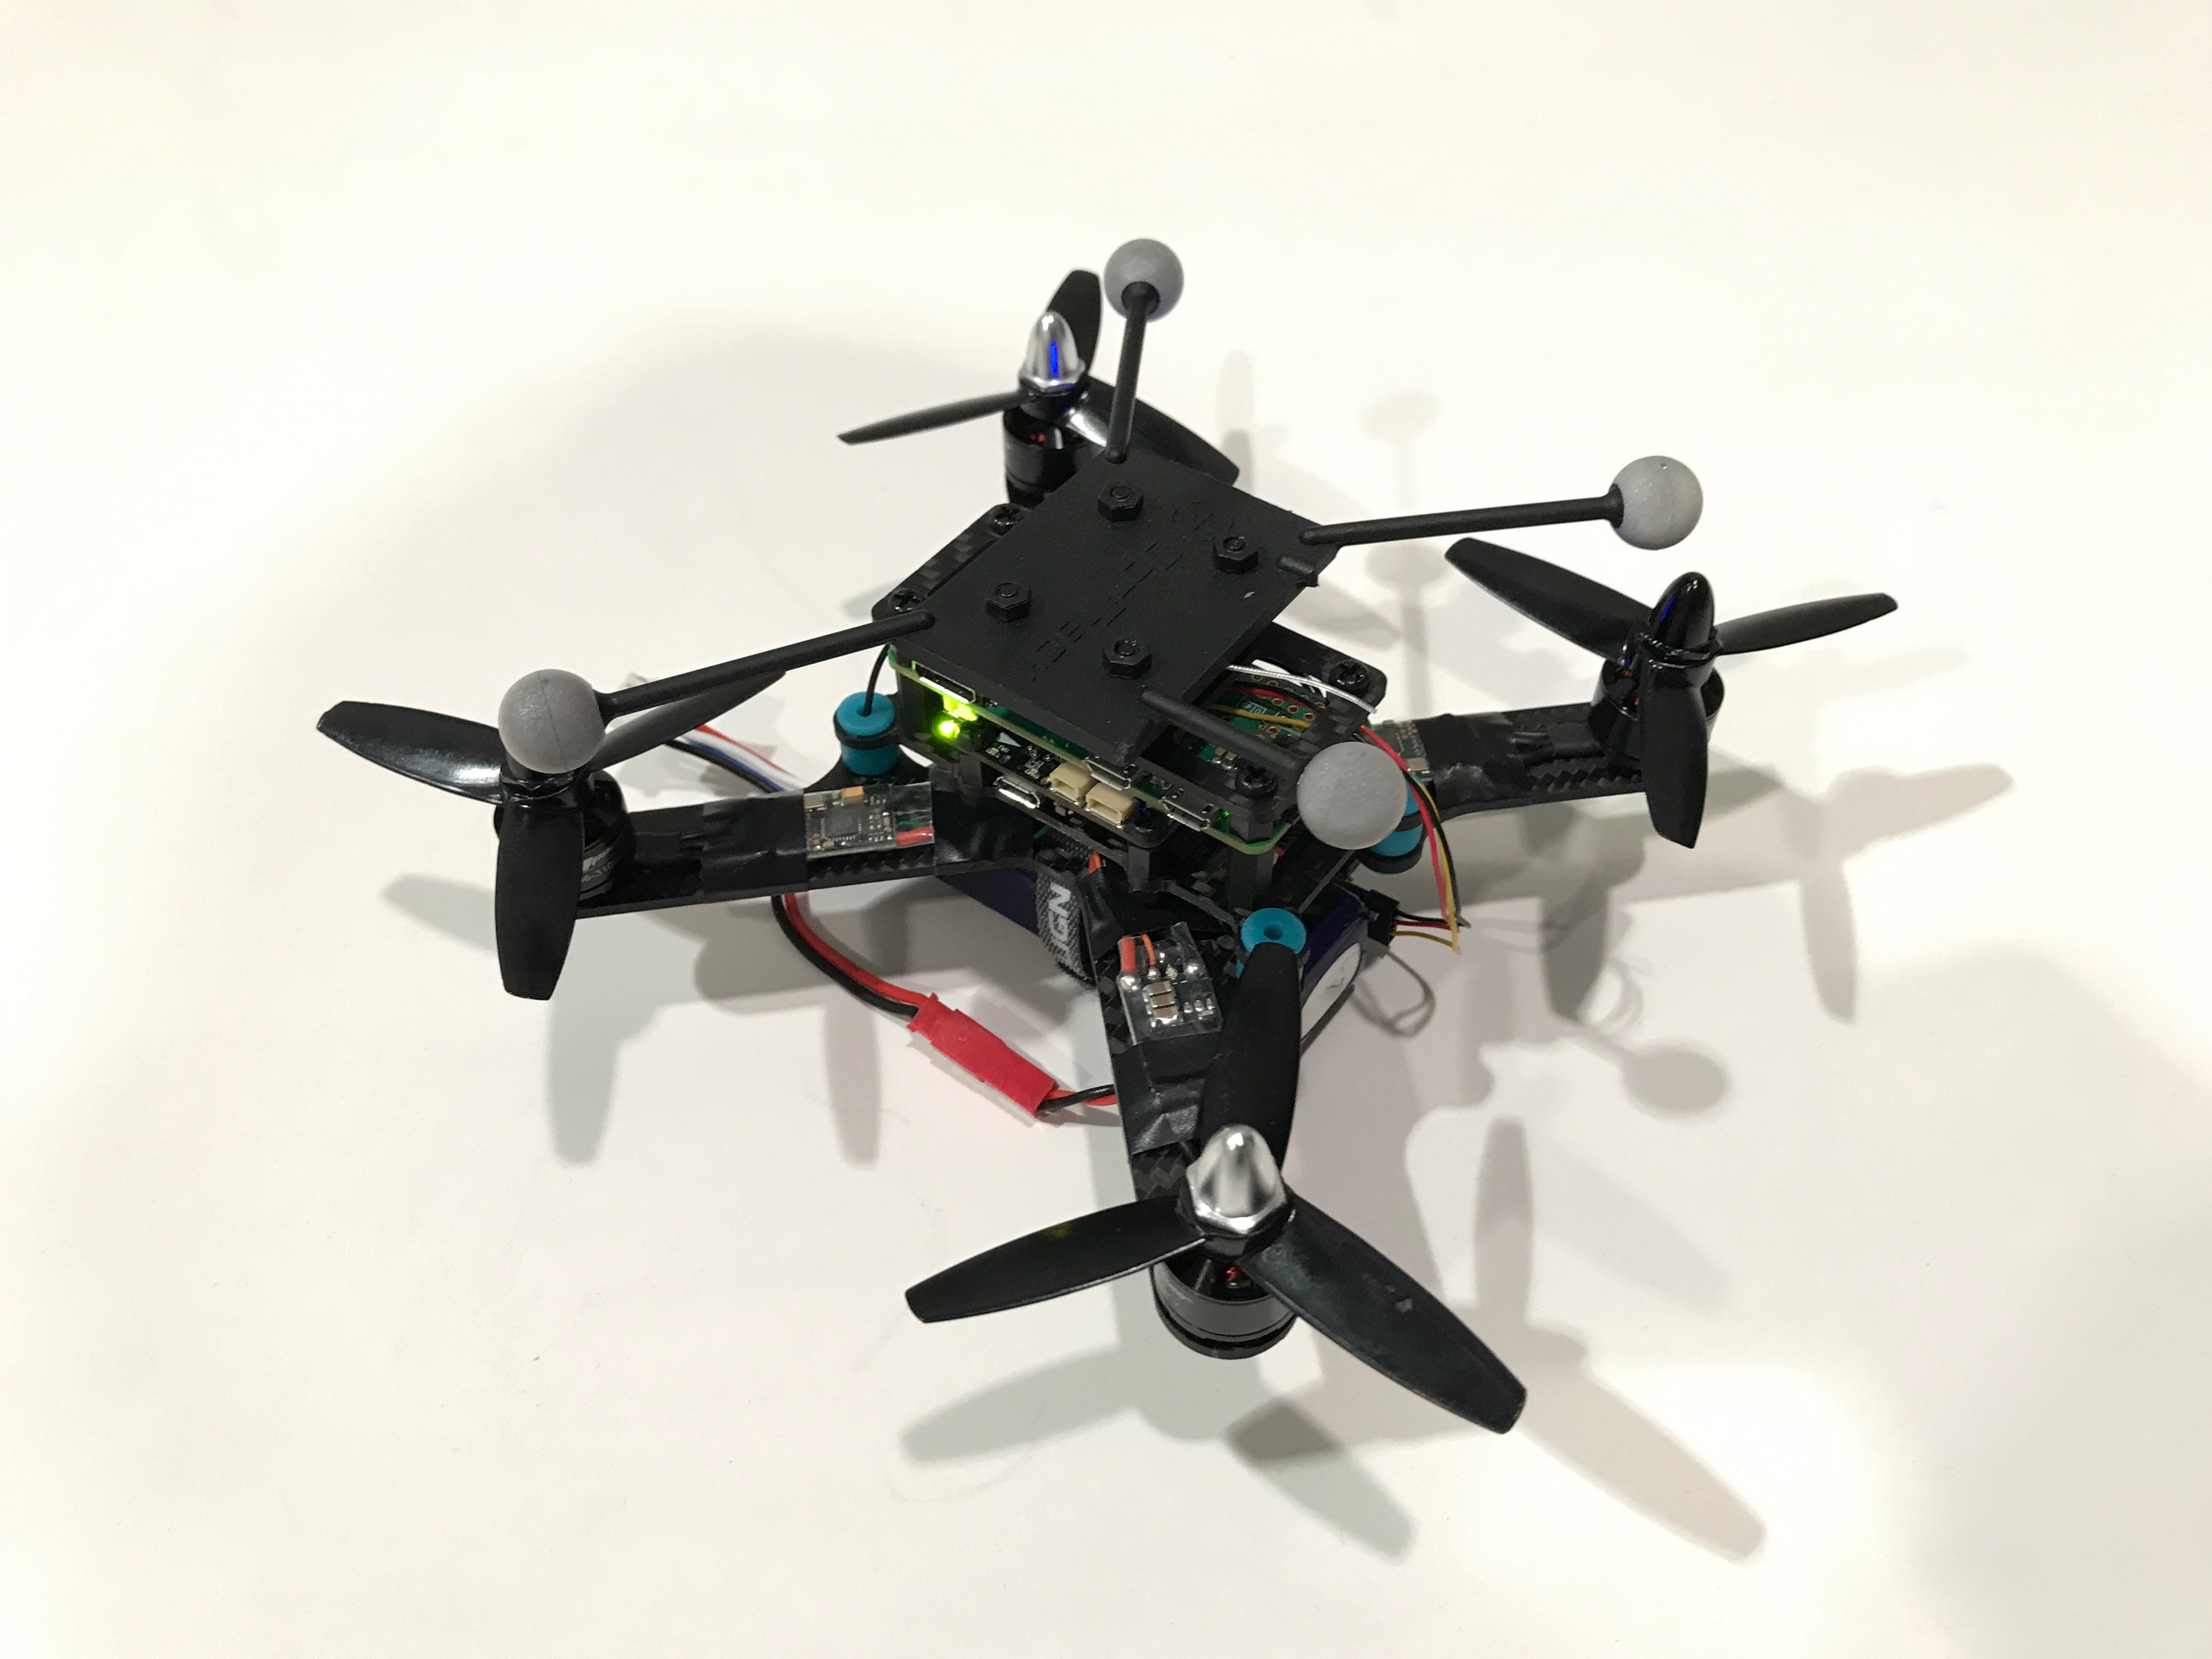
\includegraphics[width=\linewidth]{chapters/chapter-03/figures/ant1_2.jpg}
\endminipage
\caption{Ant drone}
\label{fig:ant1}
\end{figure}

\begin{figure}[!htb]
\minipage{0.5\textwidth}
  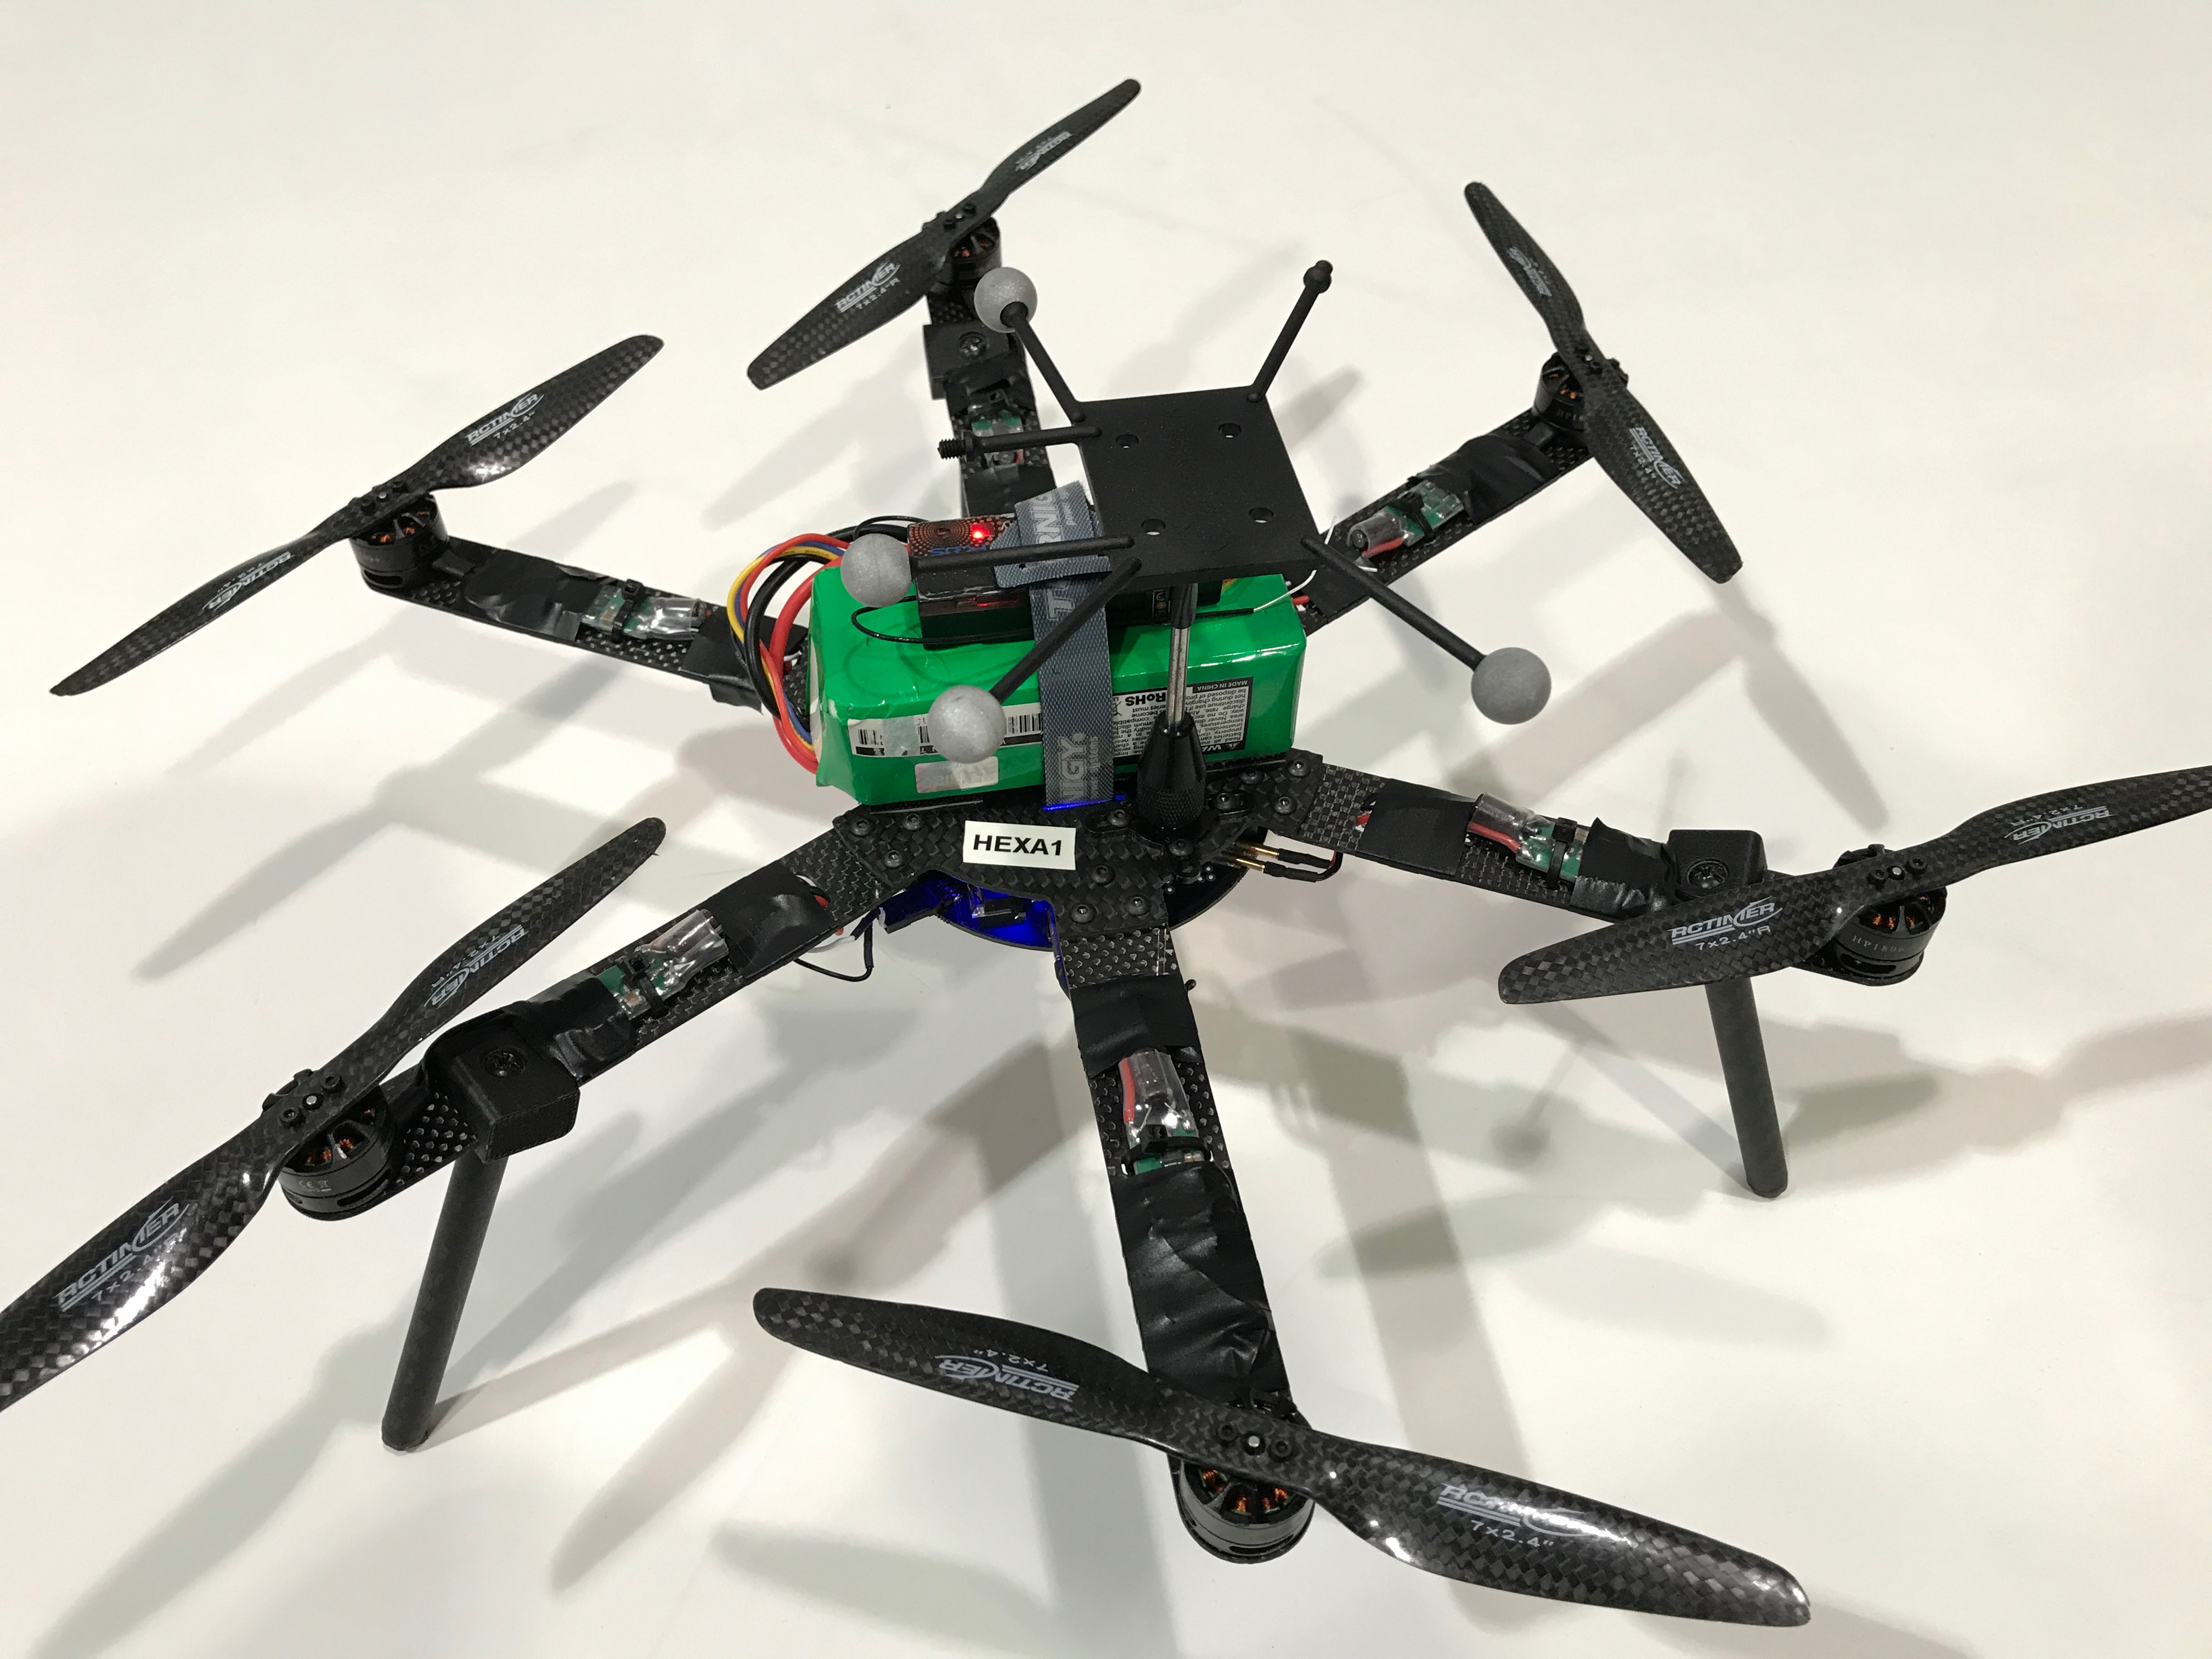
\includegraphics[width=\linewidth]{chapters/chapter-03/figures/hexa_1.jpg}
\endminipage\hfill
\minipage{0.5\textwidth}
  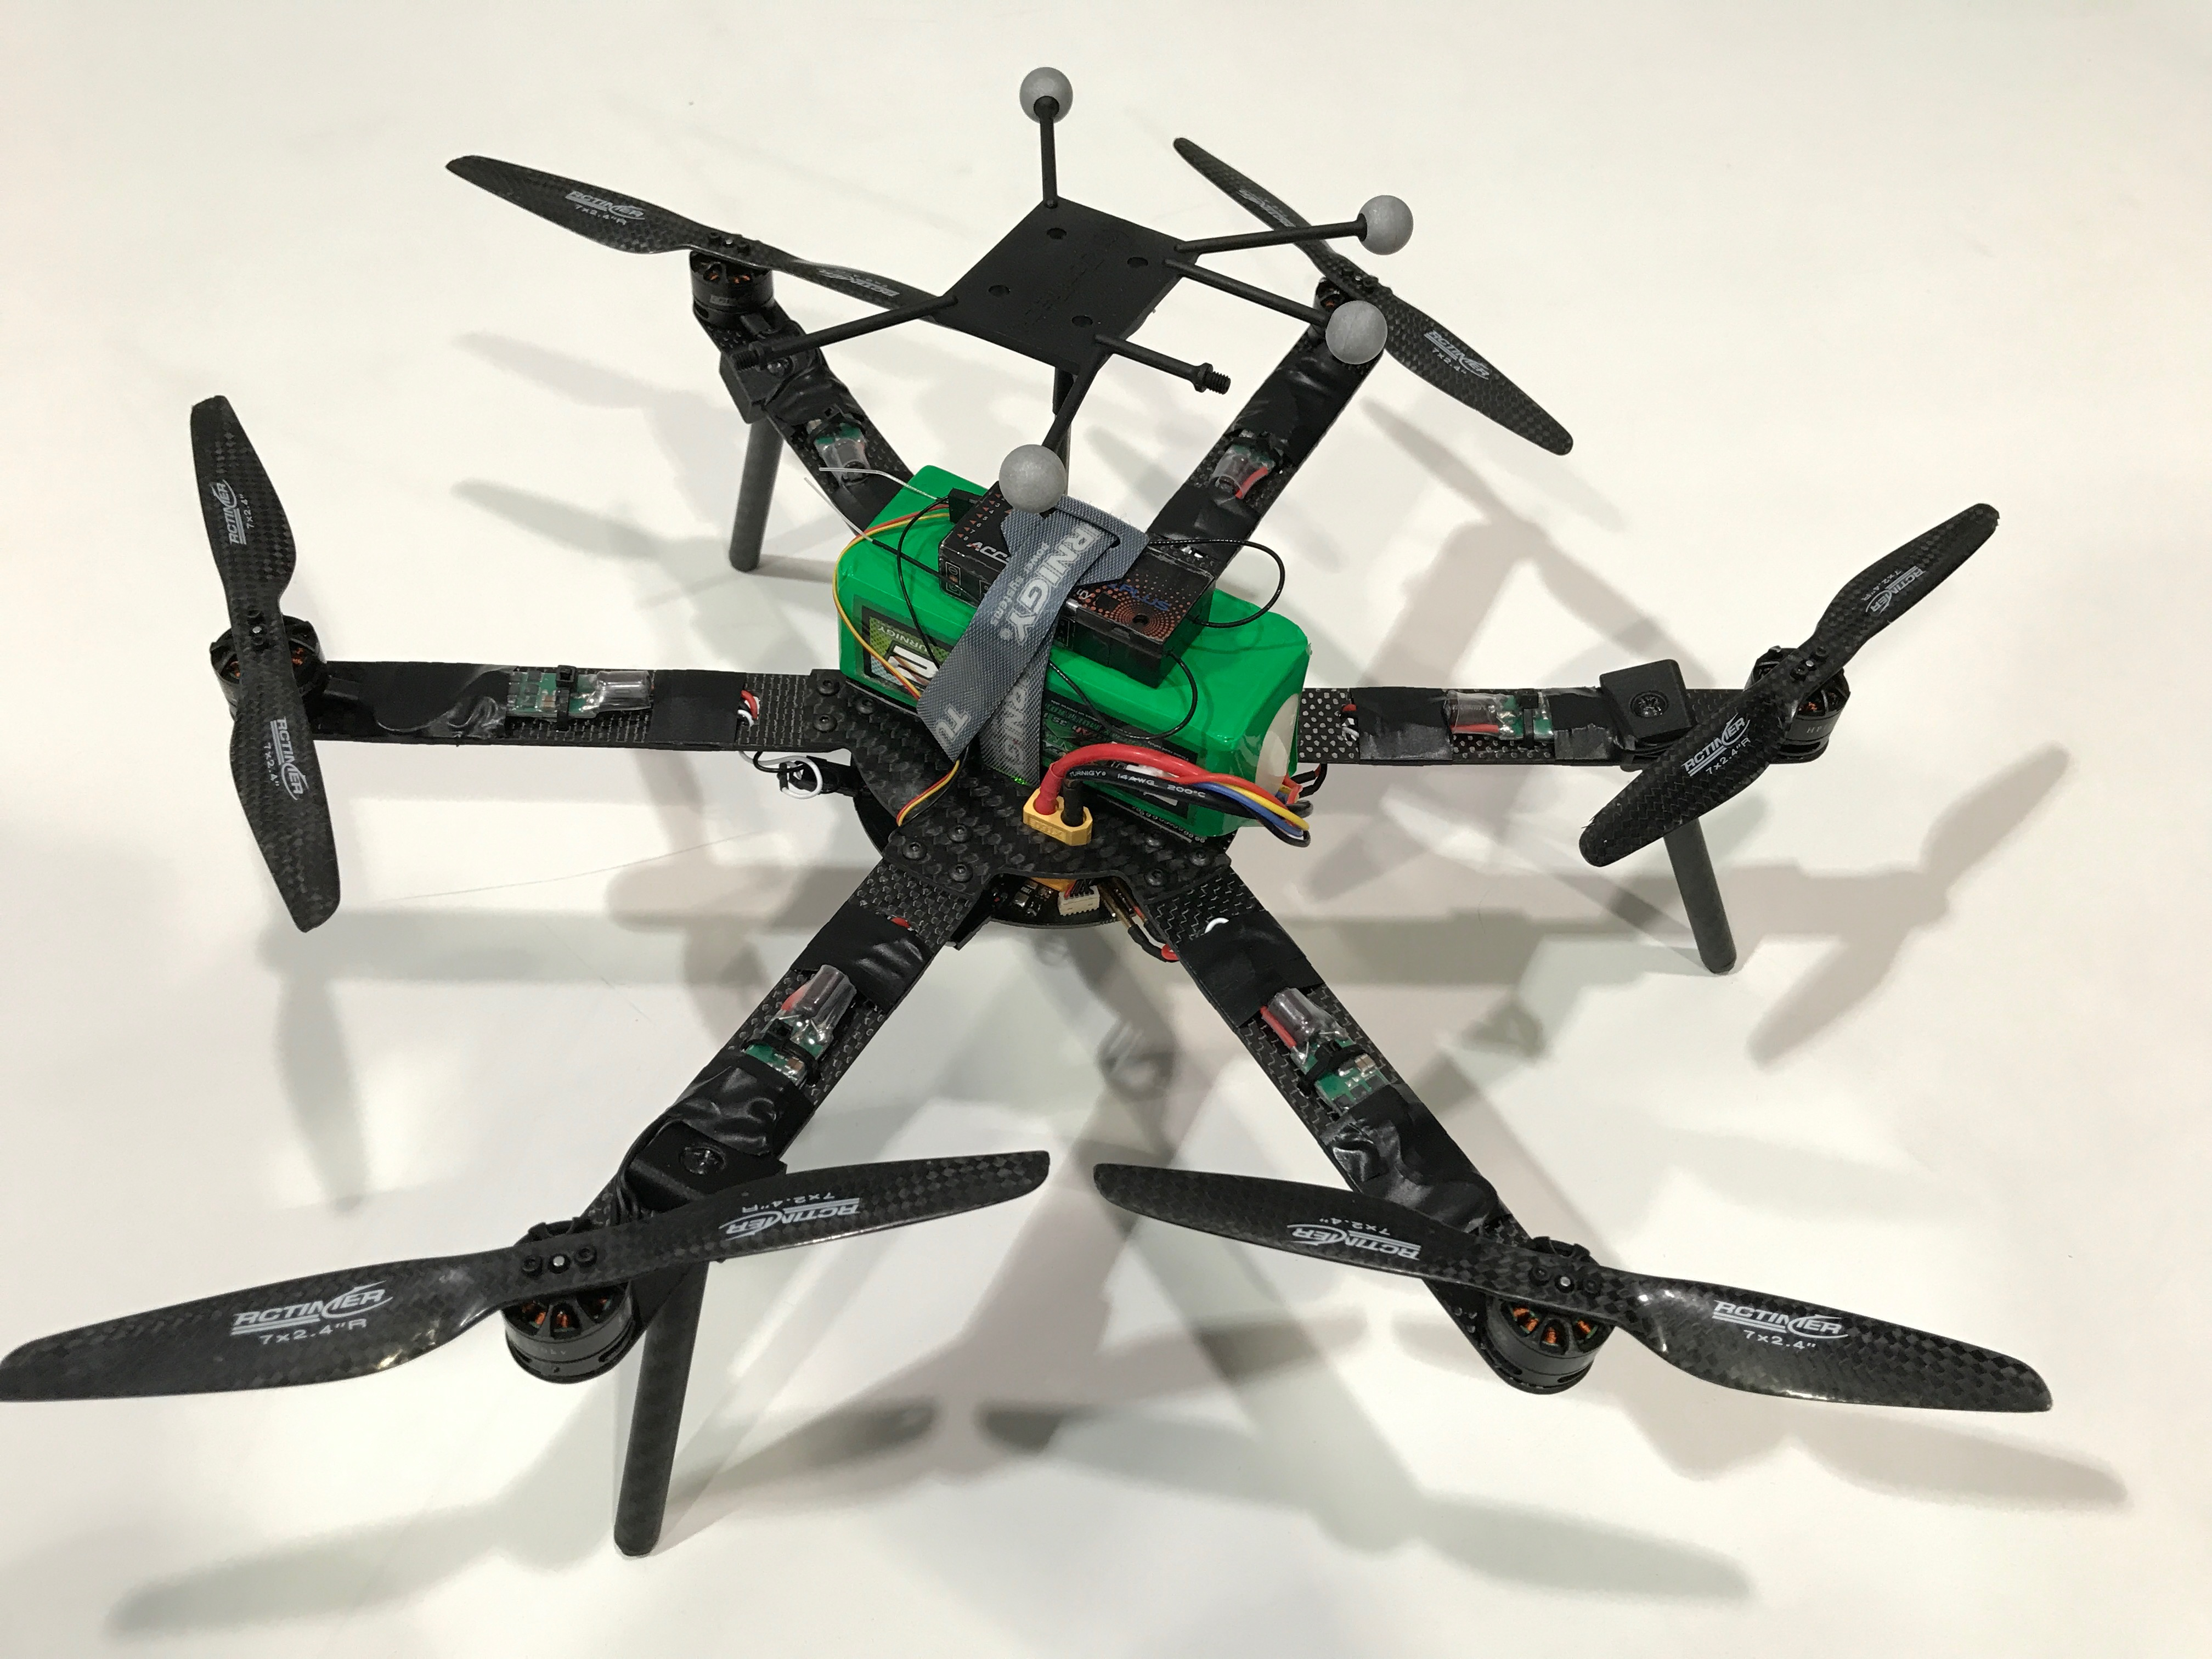
\includegraphics[width=\linewidth]{chapters/chapter-03/figures/hexa_2.jpg}
\endminipage
\caption{Hexa drone}
\label{fig:hexa}
\end{figure}
